% Instructions for Authors fuer Acta Acustica

\documentclass[twoside,twocolumn]{article}
\usepackage{acta}
\usepackage{url}
 \usepackage[utf8]{inputenc}

\begin{document}
\Eingang{00}{00}{0000} \Annahme{00}{00}{0000} \Sachgebiet{1}
\PACS{43.50.Lj, 43.50.Rq, 43.50.Qp, 43.66.Lj, 43.66.Ba}
\Band{0} \Jahr{0000} \Heft{} \Ersteseite{1} \Letzteseite{}

\AuthorsI{G. Lafay$^{1)}$, M. Rossignol$^{2)}$, N. Misdariis$^{2)}$, M. Lagrange$^{1)}$, J.F. Petiot$^{1)}$}
\AddressI{$^{1)}$ Institut de Recherche en Communications et  Cybern\'etique de Nantes (IRCCYN), Nantes, France.\\
\hspace*{8pt}gregoire.lafay@irccyn.ec-nantes.fr\\
$^{2)}$ Institut de Recherche et Coordination Acoustique/Musique (IRCAM), Paris, France}

% \footnotemark[1] \Authornotes{\footnotetext[1]{} }

\Englishtitle{Investigating soundscapes perception through acoustic scenes simulation. Part II} \Germanorfrenchtitle{}

\Kolumnentitel{Lafay et al. : Approaching mental representations}

\Englishabstract{This paper introduces a new experimental protocol to study mental representations of urban soundscapes through a simulation process. Subjects are asked to create a full soundscape by means of a  software dedicated to sound arrangement, coupled with a structured sound data set. This paradigm is used to characterize urban sound environment representations, by analyzing the sound classes that were used to simulate the auditory scenes. Three others perceptive experiments are conducted to refine the analysis of the simulated urban acoustic scenes. Results show that a semantic characterization in terms of presence~/ absence of sound sources is an effective way to characterize urban soundscapes and potentially sufficient for some description tasks.}
\Germanorfrenchabstract{}

\ScientificPaper



\newcommand{\gl}[1]{\textcolor{blue}{GL : #1}}
\newcommand{\partI}[1]{\textcolor{red}{From part I : #1}}
\newcommand{\ml}[1]{\textcolor{magenta}{ML : #1}}
\newcommand{\mr}[1]{\textcolor{green}{MR : #1}}

%%%%%%%%%%%%%%%%%%%%%%%%%%%%%%%%%%%%%%%%%%%%%%%%%%%%%%%%%%%%
%%%%%%%%%%%%%%%%%%%%   INTRODUCTION      %%%%%%%%%%%%%%%%%%%
%%%%%%%%%%%%%%%%%%%%%%%%%%%%%%%%%%%%%%%%%%%%%%%%%%%%%%%%%%%%
\section{introduction}

\partI{For two decades, the soundscape paradigm has been considered to study the perception of acoustic scenes in order to provide urban planners with meaningful sound quality indicators (see \cite{dubois2006cognitive} and  \cite{aletta2016soundscape} for extensive reviews). Most studies follow the modus operandi of cognitive psychology \cite{maffiolo_caracterisation_1999}, by first describing the soundscape using both acoustic measurements and perceptive factors, and then investigating the interactions between those descriptors to understand the cognitive processes involved in the perception of the acoustic scenes. Soundscape studies are thus interdisciplinary \cite{davies_perception_2013, aletta2016soundscape}, borrowing tools from various fields such as acoustics, psycho-physics, cognitive psychology but also psycho-linguistics, sociology and data mining.}

\partI{The soundscape approach appears to be a powerful tool to develop perceptively motivated indicators \cite{schulte-fortkamp_soundscape:_2007}. That said, the use of various experimental protocols to assess and measure soundscapes makes the integration of results difficult \cite{davies_perception_2013}. Also, there still exist no definite consensus in the soundscape community about the acoustic descriptors to be used \cite{aletta2016soundscape}. This issue prevents experimenters to provide  urban planners with generic and clear indicators or models able to predict sound environment quality \cite{schulte-fortkamp_soundscape:_2007, aletta2016soundscape}. Recently, several projects such as the European Cooperation in Science and Technology Action (TD0804: soundscape of European Cities and Landscapes) or the Positive Soundscape project \cite{davies_perception_2013} have been undertaken to standardize soundscape assessment and descriptors \cite{schulte2013soundscape}, but those matters are still considered as open problems.}

\partI{We believe that soundscapes studies greatly suffer from one important issue: to the best of our knowledge, there is no morphological definition of a soundscape, and therefore no standardized way to decompose it in distinct elements. It is thus difficult to study precisely which component of the environment is the cause of potential variations in the perceptive measurements.} The fact that sound sources does not influence the perception in a equal manner is not a novel idea. In \cite{schafer1977tuning} Schafer had already introduced the notion of \emph{soundmark}, which refers to sounds with subjective qualities that bring them into focus for people used to them. 

To tackle this issue, we introduced in the first part of this paper \cite{lafayPartI} a simulation protocol where subjects were asked to simulate a full acoustic environment thanks to a soundscape simulator linked to a dataset of isolated sound samples. The simulation allows us to generate acoustic environments fully characterized in term of both source presences and sound levels, thus enabling us to study contribution of each sound source on soundscape perception. We presented the results of a case study focused on urban soundscapes pleasantness. First a simulation experiment was run giving us 36 ideal urban soundscapes (i-scenes) and 36 non-ideal ones (ni-scenes). Second a pleasantness rating experiment was run with a different pool of subject using a 7-points semantic scale. The combined analysis of the two experiment allowed us to draw the following outcomes:

\begin{itemize}
\item The ability of the sound level to characterize the pleasantness relies upon the quality of the scene itself. For positively rated scenes (i-scenes), it is not relevant.
\item  A semantic description of the soundscapes in terms of presence~/ absence of sound sources is an effective criterion to distinguish between ideal or non-ideal urban environment.
\item  A few event markers (see Table~\ref{tab:markers}), appearing at various semantic levels, suffice to perform efficient discrimination between the ideal or non-ideal urban environment, although the type of markers found in this study may depend on the socio-cultural background of the subjects. 
\item Sound level computed on the markers better characterize the appraisal than global sound level.
\end{itemize}

Following those first results, we conducted two complementary experiments to further our understanding of the sound source contribution on scene perception:\\

\textbf{Experiment-1}: a pleasantness rating experiment similar. In order to check the effect of markers, subjects must rate 144 scenes comprising the 72 initial scenes, and the same 72 scenes but re-simulated without the sound markers of semantic level 1. The goal is to check whether markers are such salient discriminant factors that removing them will blur the distinction between i- and ni-scenes.\\

\textbf{Experiment-2}:  a free sorting task experiment. This experiment has multiples goals:
\begin{enumerate}
\item to confirm that the categorizations of the simulated scenes rely on sound sources identification. This fact has been shown considering recordings of complex sound environment mostly  \cite{maffiolo_caracterisation_1999,dubois2006cognitive}
\item to identify what sound categories are spontaneously used by the subjects to categorize the scenes, and observe at what level of abstraction those categories are expressed.
\item to see whether  the event markers  \gl{, caractéristiques de qualité d'un environnement} correlate with those categories  
\item  \gl{Autour de quelles classes/categories s'opèrent les regroupements par similarité}\\
\end{enumerate}

\gl{HERE RESULTS}

\begin{table}[t]
 \setlength{\tabcolsep}{0.1pt}
 \centering
  {\renewcommand{\arraystretch}{0.9}
\begin{tabular}{c c c c} 
Semantic   &  \multicolumn{2}{c}{Markers} \\
level & i-scenes & ni-scenes \\
\hline
0  &              &  construction work  \\
\hline
1  & church bell  & horn  \\
   & bell bike    & siren \\
   & animal       &       \\
   \hline
2  & birds         & horn  \\
   & church bell   & siren \\
   & bell bike     &       \\
   \hline
3  & birds singing & horn  \\
   & church bell   & siren \\
   & bell bike     &       \\
   & male footsteps concrete &  \\
  \hline
\end{tabular}
}
\vspace{0.5mm}
\caption{\label{tab:markers} Event classes found to be markers. In each cell, markers are ordered from top to bottom by decreasing V-test values.}
\end{table}

\section{Experiment-1 set-up}
\subsection{Task}

Subjects are asked to evaluate the pleasantness of 144 urban environments, comprising the 72 original simulated scenes, and the same 72 scenes but generated without the sound markers. Evaluation is made using a bipolar semantic scale of 11 points going from -5 (non ideal, very unpleasant) to +5 (ideal, very pleasant). The first ten scenes are used to give the subject an idea of the pleasantness range. Those scenes are repeated at the end of the experiment and their first occurrences are not taken into account for the analysis. Subject are forced to listen to at least the 20 first seconds of the scenes, but are free to skip the 10 last seconds if needed. Scenes are presented in a randomized order, but we make sure that the ten first scenes 1) contain sound markers and 2) are evenly balanced between i- and ni-scenes.

\subsection{Participants and apparatus}

12 subjects take part in experiment-1. None of them did the simulation experiment nor the first pleasantness rating experiment. The experiment is run simultaneously for the firsts 5 subjects.  The remaining of the subjects did the experiment separately. All the subjects did the experiment in a calm environment. Audio is presented diotically to each participant via \textit{BeyerDynamic DT 990 Pro} semi open headphones at -12 dB (FS). One experimenter is always present to give instructions and answer queries if needed. The experiment lasts one hour and a half. All the subjects successfully completed the experiment. 

\subsection{Statistical analysis}

We measure significance using paired Student's t-test and two-way repeated-measure ANOVA. All the tests are preformed at a $\alpha=5\%$ significance level. For repeated measures designs, sphericity is assessed using Mauchly's sphericity test. If the sphericity assumption does not hold, we use the Greenhouse-Geisser correction, and in that case the corrected $p$-value is noted $p_{gg}$. All correlations are computed using the Pearson product-moment correlation coefficient.

\section{Experiment-1 results}

Among the 12 subjects, one gives an averaged rate for the ni-scenes superior to 2*IQR of the median averaged rates of the other subjects. That subject is therefore considered as an being an outlier and  removed from the data.

Figure~\ref{fig:xp4_3}.a depicts the distributions of the averaged ratings for the i- and ni-scenes, with and without markers, considering the scenes as observations. We note that the impact of the scene outlier detection procedure run in \cite{lafayPartI} stands in this experiment: none of the i-scenes (resp. ni-scenes) has an averaged rating inferior to the maximum averaged rating of the ni-scenes. Furthermore we have a correlation of $r=0.95$ ($p<0.01$) between the scene averaged ratings of the two experiments, denoting  the consistency of the results.

We show the averaged ratings per subjects for the i- and ni-scenes with and without markers in Figure~\ref{fig:xp4_3}.b. A two way repeated measure ANOVA considering the presence of markers as well as the scene type (i/ni) as independent variables reveals significant effect of both the marker presence ($F[1,10]=14$, $p_{gg}<0.01$), the scene type ($F[1,10]=116$, $p_{gg}<0.05$) and the interaction ($F[1,10]=49$, $p_{gg}<0.01$). \emph{Post hoc} analysis shows significant differences between the mean averaged ratings with and without markers for both the ni-scenes ($p<0.01$) and  the i-scenes ($p<0.05$). 

Figures~\ref{fig:xp4_3}.c and~\ref{fig:xp4_3}.d illustrate the effect of scene type and presence/absence of markers on $LAeq$ and density, respectively. Concerning $LAeq$, a two way repeated measure ANOVA shows a significant effect of both the markers presence ($F[1,35]=123$, $p_{gg}<0.01$) and the scene type ($F[1,35]=77$, $p_{gg}<0.01$), with \emph{post hoc analysis} showing significant differences between the mean $LAeq$ for both the ni-scenes ($p<0.01$) and the i-scenes ($p<0.05$) with and without markers. Considering the densities, we also find a significant effect of both the markers presence ($F[1,35]=52$, $p_{gg}<0.01$) and the scene type ($F[1,35]=6$, $p_{gg}<0.05$), with \emph{post hoc} analysis revealing once again significant differences for both the ni-scenes  ($p<0.01$) and the i-scenes ($p<0.05$) with and without markers. Those results show us that, as expected, the removal of the markers does have an effect on scene morphology, since this operation reduces both the densities and the sound levels for both the i- and ni-scenes.

This results validates our hypothesis that the presence/absence of specific sounds classes directly influence the pleasantness of an acoustic scenes. As expected, the removal of the ni-makers increases the pleasantness of ni-scenes, by 1 in average. The removal of the i-markers does decrease the pleasantness of i-scenes, but by a lower amount (0.4), more surprisingly.

While $LAeq$ does have an influence on pleasantness, we can conclude here that sound markers are more important. Indeed, removing positive markers such as \textit{bike bell}, \textit{church bell} and \textit{birds} from a scene decreases the sound level, and should \emph{a priori} have a positive impact on pleasantness, but in fact the scene rating decreases significantly.
 
\begin{figure}[t]
\begin{center}
\includegraphics[width=\columnwidth]{../gfxMatlab/xp4_3.eps}
\caption{\label{fig:xp4_3} Boxplot of the averaged ratings considering (a) subject as observations and (b) scenes as observations. Boxplot of (c) the scene $LAeq$ and (d) the scene densities; \textit{w/ m} and \textit{w/o m} indicate the presence or absence of sound markers respectively.}
\end{center}
\end{figure}

\subsection{pleasantness and sound level}

\begin{table}[t]
 \centering
\begin{tabular}{c c c} 
            & w/ markers          & w/o markers       \\
\hline
all         & -0.82 ($p<0.01$)    & -0.79 ($p<0.01$)  \\
i-scenes    & -0.49 ($p<0.01$)    & -0.53 ($p<0.01$)  \\
ni-scenes   & -0.85 ($p<0.01$)    & -0.68 ($p<0.01$)  \\
\hline
\end{tabular}
\vspace{0.5mm}
\caption{\label{tab:plCorr} Correlations between $LAeq$ and pleasantness.}
\end{table}

To study the impact of the markers removal on how sound level is able to characterize the appraisal, we compute the correlations between $LAeq$ and the averaged pleasantness. Results are depicted in Table~\ref{tab:plCorr}.

Correlations observed for the scenes with markers confirm the trends observed in \cite{lafayPartI}. The strong correlation observed for the ni-scenes with markers and the weak correlation observed for the i-scenes reveal that 1) sound level does not characterize appraisal in a equal manner for the i- and ni-scenes and 2)  while sound level is a good descriptor of pleasantness for ni-scenes, it is not the case for positively rated ones.

Moreover results show that removing the markers tends to slightly increase the correlation for the i-scenes, and decrease the correlation for the ni-scenes. Considering the i-scenes, we sow in \cite{lafayPartI} that the louder the i-markers relative to the remaining of the sounds, the higher the pleasantness. It appears that in absence of the i-markers, the negative influence of the sound level on the appraisal becomes more predominant. Considering the ni-scenes, the inverse effect is observed. Indeed results of \cite{lafayPartI} showed a strong negative correlation between the $Laeq$ of the ni-markers and the pleasantness. It appears here that the removal of those markers drastically diminishes the negative impact of the sound level.

These results are strong indicators that all the sources do not equivalently participated in pleasantness perception. In particular they show that the ability of sound level to predict pleasantness is only due to the presence of some sources, \emph{i.e.} the ni-markers. In the absence of such sources, appraisal seems to rely on other descriptors.

 

\section{Experiment-2 set-up}
\subsection{Task}
Les mêmes resultats sont observé dans \cite{guyot2005urban, ricciardi2015sound}.

Subjects are asked to group the 72 simulated scenes (36 i-scenes and 36 ni-scenes) based on their similarity. They are allowed to create as many clusters as they wish. The scenes are represented as dots on a plane. Subjects may listen to a scene by clicking on a dot, move the dots, and use color to specify clusters. After the  sorting part, subjects are asked to label each cluster using a word, a list of words, or a short sentence. 

\subsection{Participants and Apparatus}

Experiment-2 is run with the same subjects who took part in the rating experiment in \cite{lafayPartI}, but two weeks after. The 10 subjects  take part in the experiment simultaneously, in a calm environment. Audio is presented diotically to each participant via \textit{BeyerDynamic DT 990 Pro} semi open headphones at -12 dB (FS). One experimenter is always present to give instructions and answer queries if needed. All the subjects successfully completed the experiment.  

\subsection{Statistical analysis}

We measure significance using one way. All the tests are preformed at a $\alpha=5\%$ significance level. For multiple comparison procedures we use Bonferroni correction, and in that case we designate by $p_{bonf}$  the corrected $p$-value. All correlations are computed using the Pearson product-moment correlation coefficient.

\section{Experiment-2 results}
\subsection{Categorization strategies}

\setlength\tabcolsep{0.7mm}
\begin{table}[t]
 \centering
{\renewcommand{\arraystretch}{0.9}
\begin{tabular}{lccccc}
subject & source & location & quality & volume & frequency  \\
\hline
    $1^*$&        &          &    x    &        &           \\
    2    &   x    &          &         &        &           \\
    $3^*$&        &          &         &    x   &     x     \\
    4    &   x    &          &    x    &        &           \\
    5    &   x    &    x     &    x    &        &           \\        
    $6^*$&        &          &    x    &        &           \\
    7    &   x    &          &         &    x   &           \\
    $8^*$&        &          &    x    &        &           \\
    9    &   x    &    x     &         &        &           \\
    10   &   x    &          &         &        &           \\
\hline
\end{tabular}
}
\vspace{0.5mm}
\caption{\label{tab:StratSate} Strategies adopted by the subjects to categorize the scenes. Subjects removed from the data are indicated by $*$.}
\end{table}

\setlength\tabcolsep{0.7mm}
\begin{table}[t]
 \centering
{\renewcommand{\arraystretch}{0.9}
\begin{tabular}{ccc}
labels & categories  & classes\\
       & (merging)   &        \\
\hline
alarm (2)             & alarm            &  \textit{car\_fire\_alarm} (sl-1) \\

horn  (2)             & horn             &  \textit{horn} (sl-1)             \\
                      & (siren/horn)     &                                    \\
siren (3)             & siren            &  \textit{siren} (sl-1)            \\
                      & (siren/horn)     &                                    \\
birds (4)             & birds            &  \textit{birds} (sl-2)             \\
\hline
church bell (4)       & church bell      &  \textit{church bell} (sl-1)      \\
church (2)            &                  &                                   \\
\hline
mechanical            & construction     &  \textit{hand tool} (sl-1)       \\
public work  (4)      &                  &  \textit{power\ tools} (sl-1)   \\
tools                 &                  &  \textit{jackhammer} (sl-1)       \\
                      &                  &  \textit{metal\_work} (sl-1)       \\
			          &                  &  \textit{vehicle\_work} (sl-1)     \\  	
\hline			                                                             
human (4)             & human            &   \textit{voice} (sl-0)           \\      
people, crowd         &                  &   \textit{footstep} (sl-1)       \\      
footstep (2)          &                  &                                   \\  
\hline
traffic (2)           & traffic          &  \textit{scooter} (sl-1)         \\
car (2)               &                  &  \textit{motorcycle} (sl-1)       \\
                      &                  &  \textit{car} (sl-1) \textit{truck} (sl-1) \\ 
\hline
water, rain (2)       & water            &   \textit{water}$^T$ (sl-1)          \\ 
bad weather           &                  &                                  \\ 
\hline
market                & market           &   \textit{market}$^T$ (sl-1)          \\ 
                      & (human)          &                                    \\
park                  & park             &   \textit{park}$^T$ (sl-1)           \\ 
                      & (bird)           &                                    \\
nature (3)            & nature           &   \textit{nature}$^T$ (sl-0)          \\  
background$*$         & ---              &    ---                              \\ 
noise$*$ (2)          & ---              &    ---                              \\               
\hline
\end{tabular}
}
\vspace{0.5mm}
\caption{\label{tab:association}  Associations made between labels, categories and classes of the class taxonomy taken at specific semantic levels (sl). Numbers in parentheses indicate the number of subjects who use this label. ($*$) indicates labels not taken into account in this study. ($^T$) indicates texture classes}
\end{table}

From the labels used by the subjects to describe their clusters, 5 categorisation strategies can be identified (Table~\ref{tab:StratSate}). Most subjects ($70\%$) choose to categorize the scenes based on the presence/absence of sound sources. Other strategies rely on location (ex: ``\,park\,'', ``\,market\,''), affective quality (ex: ``\,calm,'', ``\,relaxing\,'', ``\,annoying\,''), volume (ex: ``\,loud\,'') and frequency (ex: ``\,presence of bass frequencies\,'').  This first result confirms previous findings showing that the categorization process relies mostly on sound source identification \cite{dubois2006cognitive,maffiolo_caracterisation_1999}, and is in line with previous studies stating that quality and location play a role in soundscape categorization \cite{aletta2016soundscape}.

\gl{Validation Claim 1}

To ensure the consistency of the analysis, we remove from the study the 4 subjects who do not use the ``\,sound source\,'' strategy, and only keep the source and location labels given by the remaining subjects to describe their clusters. 

\subsection{From labels to sound source categories}
\label{sec:fromLab2Cat}

\begin{figure*}[t!]
\centering
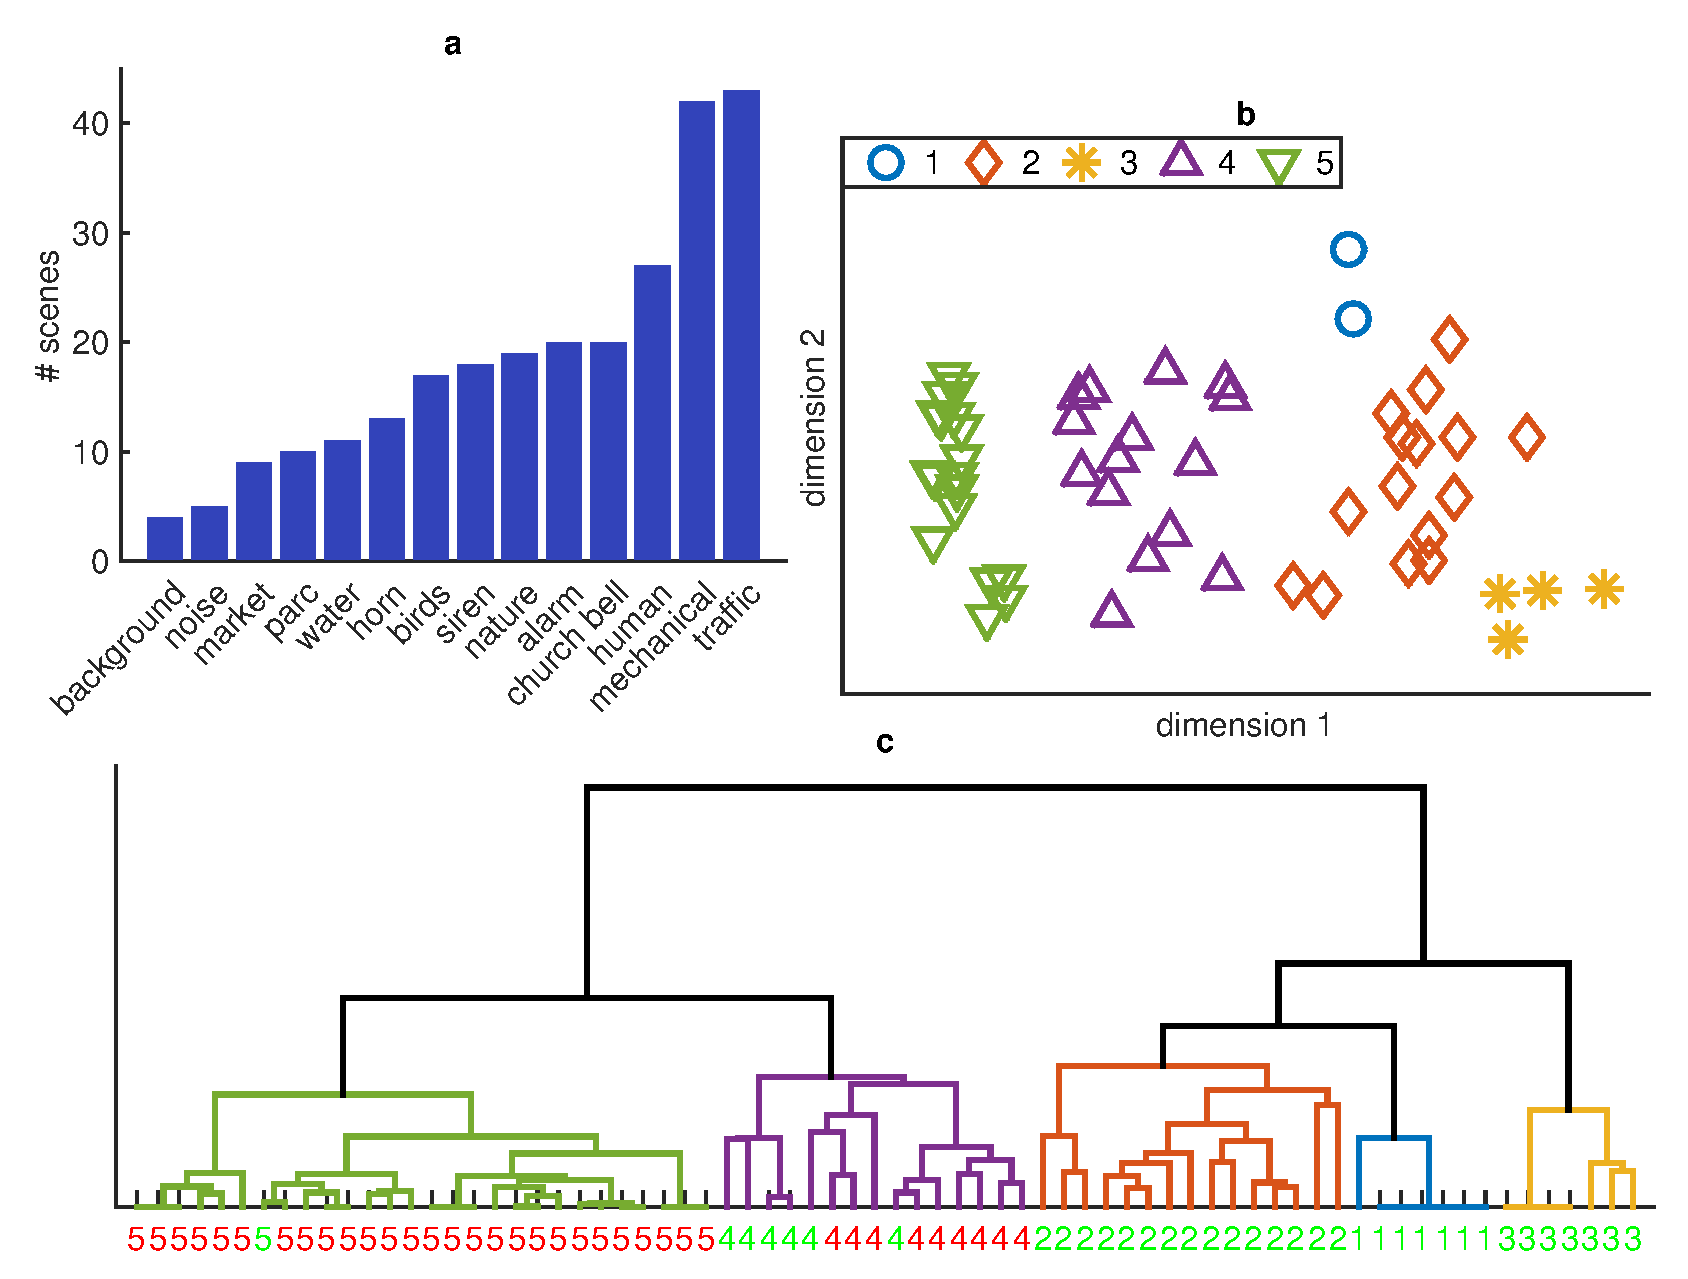
\includegraphics[width=.8\paperwidth]{../gfxMatlab/xp3_1.eps} 
\caption{\label{fig:xp3_1} (a) Number of time each semantic category has been used to describe a scene; (b) two-dimensional plot of the dimensions 1 and 2 resulting from the MDS analysis with cluster membership; (c) dendrogram resulting of the HCA analysis, x label digits indicates cluster membership while x label colors indicate scene type (green: ideal, red: non-ideal).}
\end{figure*}

We first analysed the labels used by the subjects to describe their clusters. From the descriptions, 23 labels can be isolated (see Table~\ref{tab:association} first column). The labels that designate a same sound source are then grouped into 14 categories (see Table~\ref{tab:association} second column).   

Among the 14 categories obtained, 12 of them can be directly linked with sound sources and 2 are referring to ambiguous sounds (``\,noise\,'' and ``\,background\,''). To measure the relative importance of the categories in the categorization process, we count the number of time each category has been used to describe a scene (Figure~\ref{fig:xp3_1}.a). As the categories ``\,noise\,'' and ``\,background\,'' are only used to describe less than 5 scenes, we remove them from the analysis.

It can be seen that some general categories may encompassed others (``\,human\,''>``\,market\,''), which may suggest that two subjects could have designate a same object using different levels of abstraction/specificity. In order to check that each category is effectively used to designate a specific sound source, we count the number of time two categories co-occurred in a same scene. A co-occurrence rate of $100\%$ is obtained for 3 categories associations, namely:  ``\,park\,''$\subset$``\,bird\,'', ``\,market\,''$\subset$``\,human\,'', ``\,horn\,''$\subset$``\,siren\,''. As a results, those categories are merged (see Table~\ref{tab:association} second column). It has to be noted that the co-occurence rates of the associations ``\,water\,''/``\,nature\,'' and ``\,nature\,''/``\,water\,'' are of $36\%$ and $21\%$, showing that those two categories refer to two distinct sound objects.

The remaining 9 categories show that sound source identification operates at diverse semantic levels, from the general (``\,construction\,'', ``\,human\,'') to the specific (``\,horn\,'', ``\,siren\,'', ``\,market\,''). For some categories, as for example  ``\,human\,'',  it seems that subjects mostly choose a higher abstraction level (close to semantic level 1 of the taxonomy) to describe human presence, not needing to distinguish between footsteps or voice noises. The fact that the sound reveal human activity seems to be a sufficient descriptor.

There is a considerable overlap between the event markers of the i- and ni-scenes extracted by statistical analysis (see Table~\ref{tab:markers}), and the categories spontaneously used by the subjects to categorize the scenes. Indeed among the 8 categories that could be linked to our event sound classes (only texture classes could be connected with the category ``\,water\,'' ), 4 are directly linked with \emph{event markers} of semantic level 0 and 1: ``\,horn/siren\,'', ``\,construction\,'', ``\,birds\,'' and ``\,church bell\,''. The marker \textit{male footsteps concrete} is comprised in the category ``\,human\,'', although this category may encompass other human sounds.  Of the event markers identified, only  \textit{bell bike} does not appear in the labels used by subjects.  

\gl{Les marquers, trouvés comme étant caractéristique de la qualité d'un environnement, semblent donc aussi intervenir dans un processus plus large de categorization. D'un autre coté, trois classes qui ne semblaient pas jouer de role prédominant dans la distinction des scènes idéales et non idéales font ici leur apparition (``\,traffic\,'', ``\,nature\,'' and ``\,alarm\,''), parmi elles, la categorie traffic semble avoir joué un role important dans la similarité inter-scene, celle-ci charactérisant à elle seule plus de 40 scènes.}
 
\gl{Validation Claim 2}
\gl{Validation Claim 3}

\subsection{Averaging the categorizations}

In order to gain a better understanding of the way in which class presence\,/ absence affects scene similarity, we generate an ``\,average\,'' of the clusterings performed by the subjects. For each participant, a similarity matrix $\delta_{i,j}$ is defined as: \\

\begin{itemize}
\item $\delta_{i,j}=1$ if scenes $i$ and $j$ are in the same cluster, \\
\item $\delta_{i,j}=0$ otherwise.\\
\end{itemize}

A global similarity matrix is computed by summing the individual similarity matrices, then submitted to a nonmetric  Multi-Dimensional Scaling (MDS) analysis using squared stress1 criterion and 10 replications. A 2-dimensional solution is chosen ($stress=0.07$). To make the emerging clusters explicit, we apply Hierarchical Clustering Analysis (HCA) using average between-groups linkage, with a Euclidean distance metric. HCA analysis is run for 3 to 10 clusters, and a clustering evaluation using the silhouette criterion gives us an optimal number of clusters of 5. Cluster cardinalities are shown on Table~\ref{tab:ClustersHCA}. A two-dimensional plot of the scenes coordinates obtained from the MDS analysis, also showing cluster memberships, is shown on Figure~\ref{fig:xp3_1}.b and the dendrogram resulting of the HCA analysis is shown on Figure~\ref{fig:xp3_1}.c. 

\subsection{Using sound categories and sound classes to characterize the markers}

\begin{figure*}[t!]
\centering
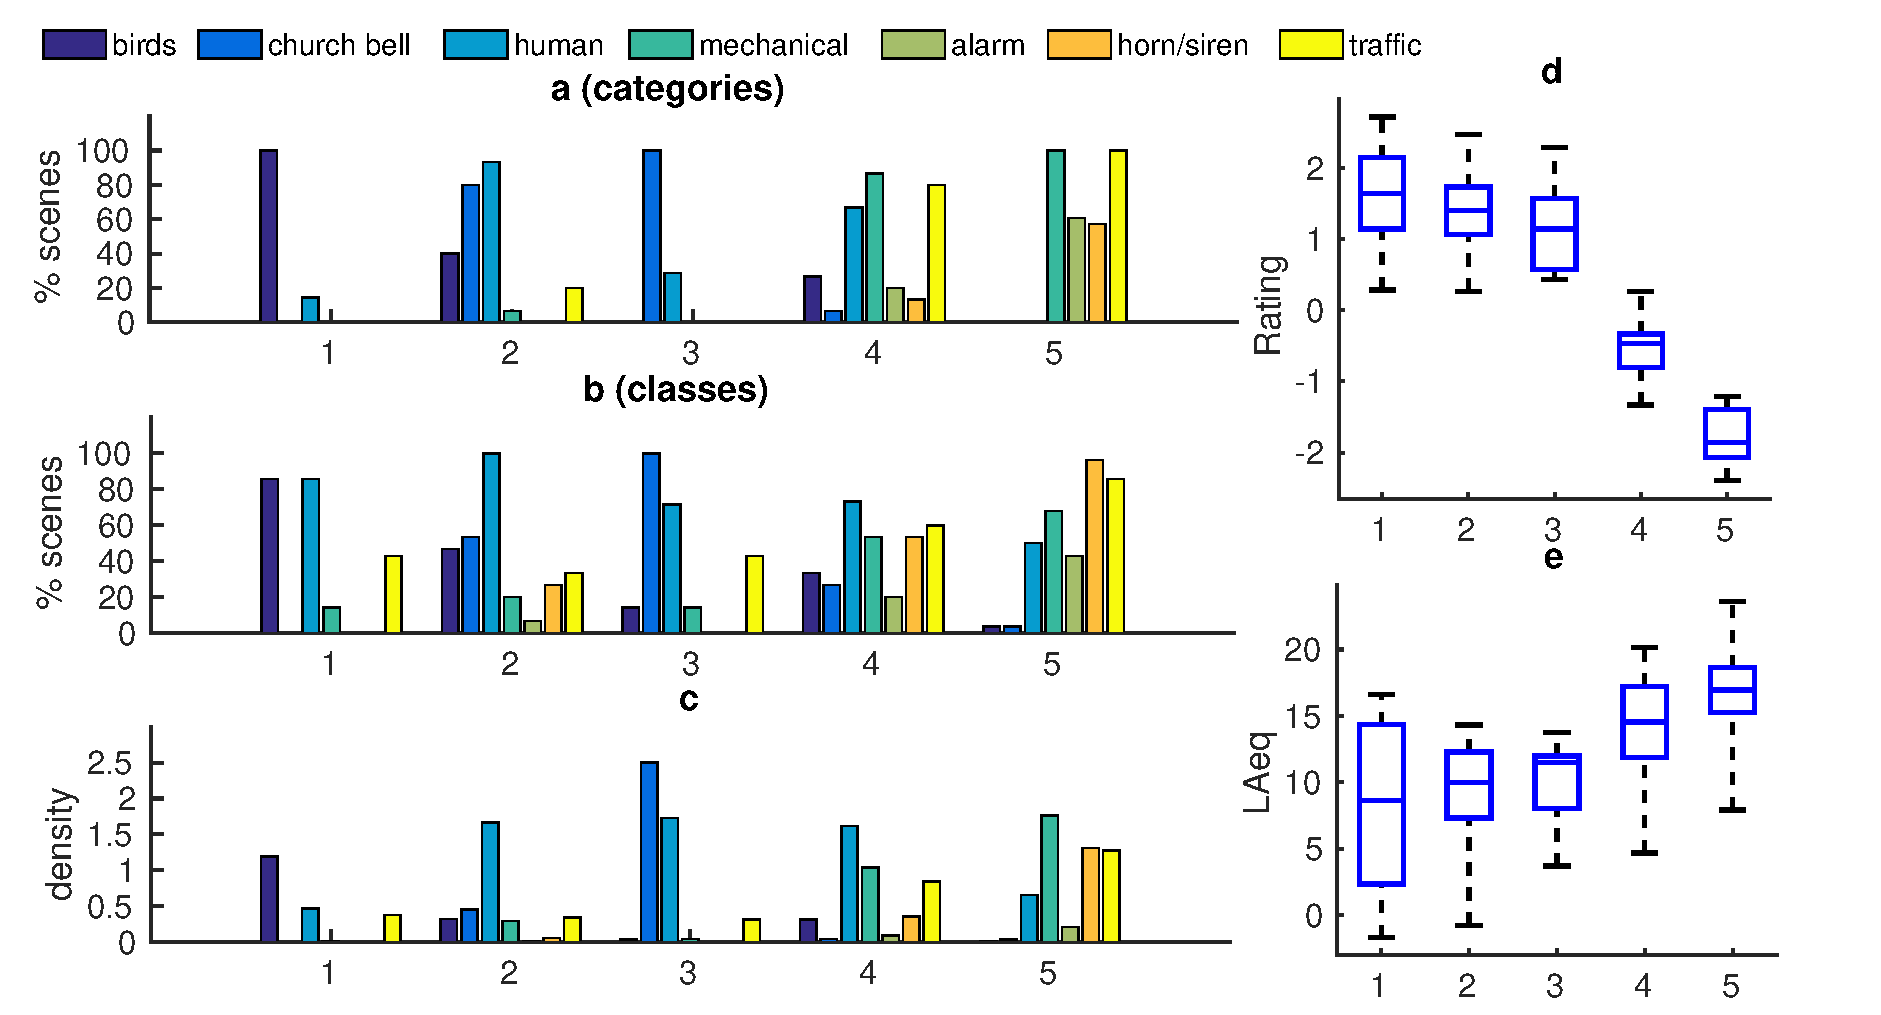
\includegraphics[width=.8\paperwidth]{../gfxMatlab/xp3_2.eps} 
\caption{\label{fig:xp3_2} For each HCA cluster: (a) Percentage of scenes described by each category; (b) Percentage of scenes simulated using the classes connected to each category; (c) Averaged densities computed considering only the samples belonging to the classes connected to each category; (d) Boxplot of averaged rates resulting of experiments-2 (observations: subjects); (d) Boxplot of averaged $LAeq$ (observations: scenes). For ease of reading, ``\,horn\,'' and ``\,siren\,'' are grouped together.}
\end{figure*}

Since the protocol based on scene simulation lets us know exactly what sound sources are present in the scenes, we can confront the categorization based on sound sources with our analysis of that ground truth.

The categories found in section ~\ref{sec:fromLab2Cat} gives us indications on the sound classes as well as the semantic levels to use to describe the clusters. The chosen sound classes are indicates in Table~\ref{tab:association}.  The descendants of sound classes linked with a category label used by subjects to categorize scenes cover $XX\%$ of the taxonomy at level 3, which shows that a great majority of sound sources are used by listeners in the appreciation of a scene, albeit at various levels of abstraction.


The percentage of scenes labeled with each semantic category (Figure~\ref{fig:xp3_2}.a) is computed for each cluster, as well as the percentage of sound classes (Figure~\ref{fig:xp3_2}.b). Small anomalies, \textit{i.e.} when a label is given and the corresponding class is absent, may be due to 1) the influence of the texture sounds, where some events may be detected, or 2) the fact that subjects may describe clusters using sources that are present in most scenes but not all of them. 
 
\gl{description categories}

Considering the categories, Figure~\ref{fig:xp3_2}.a  shows that two of the clusters resulting from the HCA analysis are formed based on the presence of one category: $100\%$ of the cluster-1 scenes are labelled ``\,birds\,'' and  $100\%$ of the cluster-3 scenes are labelled  ``\,church bell\,''. The remaining clusters seems to be characterized by a combination of multiple categories: clusters-2  ``\,human\,'' ($93\%$) $+$  ``\,church bell\,'' ($80\%$),  clusters-4  ``\,human\,'' ($67\%$) $+$  ``\,construction\,'' ($87\%$) $+$ ``\,traffic\,'' ($80\%$)   and clusters-5  ``\,construction\,'' ($100\%$) $+$ ``\,traffic\,'' ($100\%$) $+$ ``\,alarm\,'' ($61\%$) $+$ ``\,horn/siren\,'' ($57\%$). 

\gl{description classes, combien texture, combien event}

\gl{Confrontation}

The ``\,traffic\,'' category exhibits a peculiar behaviour: while classes belonging in that category are present in all clusters, it only appears when the classes \textit{horn} and  \textit{siren} are present in the cluster. This seems to indicate that traffic noises are only considered a nuisance above a certain threshold, and that moderate traffic is accepted as an integral part of an ordinary urban soundscape.

\gl{Validation Claim 5}

\subsection{Categorization based on sound source influence pleasantness and sound level}

As can be seen on Figure~\ref{fig:xp3_1}.c, scene clusters mostly obey the ideal~/ non-ideal distinction: clusters 1-2-3 contain exclusively i-scenes and cluster 5 is made up of $96\,\%$ ni-scenes, while cluster 4 is the only mixed one, with $40\,\%$ i-scenes. A cursory examination shows that this observation carries on to scene descriptions, since the event classes used to characterize scenes in clusters 1-2-3 are mostly positively connotated, whereas for those in cluster 5, all labels are characteristic of ni-scenes, while cluster 4 seems mixed.

To quantify the appraisal of the clusters, the mean average ratings from the rating experiment of \cite{lafayPartI} are computed individually for each cluster (Figure~\ref{fig:xp3_2}.d). A one-way repeated measure ANOVA shows a significant effect of the clusters on the mean averaged rates ($F[4,36]=21, p<0.01$), but \emph{post hoc} analysis shows significant effects only between clusters 1-2-3 vs 4, 1-2-3 vs 5 and 4 vs 5. It therefore seems that, from the point of view of pleasantness, the combinations of semantic categories characterizing clusters 1-2-3 are equivalent. Cluster 4 paints a more complex picture: the occasional presence of i-scene markers (``\,church bell\,'', ``\,birds\,'') and the high density of events belonging to the ``\,human\,'' category operate a clear distinction with the scenes of cluster 5, which are mostly characterized with ni-scene markers. This mixed composition of cluster 4 is reflected in the average pleasantness rating, with a score falling between those of clusters 1-2-3 and that of cluster 5. This observation suggests that adding positively connotated sounds to an \emph{a priori} unpleasant environment can improve its overall pleasantness.

A similar study bearing on the scene acoustic level $LAeq$ (Figure~\ref{fig:xp3_2}.e) yields congruent results ($F[4,67]=234$, $p<0.01$; post hoc analysis: $p_{bonf}<0.01$ for clusters 1-2-3 \emph{vs} 4, 1-2-3 \emph{vs} 5 and 4 \emph{vs} 5). Results indicate that not only does averaged pleasantness of the clusters correlate to their averaged acoustic level, but the latter also seems to be influenced by the type of sources making up the scene.

%%%%%%%%%%%%%%%%%%%%%%%%%%%%%%%%%%%%%%%%%%%%%%%%%%%%%%%%%%%%
%%%%%%%%    DISCUSSION AND PERSPECTIVES   %%%%%%%%%%%%%%%%%%
%%%%%%%%%%%%%%%%%%%%%%%%%%%%%%%%%%%%%%%%%%%%%%%%%%%%%%%%%%%%

\section{Conclusions and perspectives}

From the outcome of experiment-2, we conclude that:

\begin{itemize}
\item Sound scene categorization relies greatly on sound source identification.
\item Identification takes places at several semantic levels, and mostly hinges on 8 well-defined categories: ``\,church bell\,'', ``\,birds\,'', ``\,human\,'', ``\,horn\,'', ``\,siren\,'', ``\,alarm\,'', ``\,construction\,'', ``\,traffic\,''.
\item The scene markers coincide greatly with the categories spontaneously used by subjects to describe and characterize scene clusters.
\end{itemize}



\noindent \textbf{Acknowledgements}\\
\setlength{\parindent}{0.7cm} 
Research project partly funded by ANR-11-JS03-005-01. The authors thank the students of the Ecole Centrale de Nantes for their willing participation.

%----------------------------------------------------------------------------------------
%	REFERENCE LIST
%----------------------------------------------------------------------------------------


\References{}{../biblio}{actalit}



\end{document}
